\chapter{Руководство пользователя} %todo стянуть с документации к NCC
\label{ch:usrmanual}

Разрабатываемый сервис агрегации данных по call-центру входит в состав Naumen Contact Center и поставляется вместе с ним же.
Поэтому, для общих моментов в текущем разделе будет приведено руководство пользователя по NCC\@.

\section{Установка}

%\subsection{Установка Oracle Linux 7.X} todo если будет мало текста -- раскоменнтировать и добавить недостающие пункты https://callcenter.naumen.ru/docs/ru/ncc73/ncc/web/Content/Installation/Server_OS_Installation/Linux_Oracle_Installation_Kickstart.htm

%На каждый сервер NCC должна быть установлена последняя версия ОС Oracle Linux 7.х.
%Данное описание предполагает использование сценария установки (KickStart) и описывает минимальные действия, необходимые для установки ОС Oracle Linux 7.х.
%
%Версия операционной системы Oracle Linux должна быть не ниже версии 7.2.
%
%Дистрибутив Oracle Linux доступен на сайте Oracle (https://edelivery.oracle.com/linux) после предварительной регистрации.
%
%Для установки ОС выполните следующие действия:

Naumen Contact Center устанавливается при помощи мастера установки, работа с которым осуществляется посредством Web-интерфейса.

Для установки выполните следующие действия:
\begin{enumerate}
    \item подключитесь к мастеру установки: откройте интернет-обозреватель и перейдите по адресу \texttt{https://hostname:8001}, где \texttt{hostname} — IP-адрес сервера, на который был установлен пакет \texttt{ncc-installer};
    \item подключитесь к системе Server Access: Укажите имя пользователя и пароль для доступа к личному кабинету системы Server Access;
    \item укажите параметры инсталляции, если на рабочих местах операторов используется операционная система Ubuntu Linux, установите флажок Установить NSP репозиторий;
    \item укажите параметры соединения для серверов и баз данных;
    \item мастер запустит ряд проверок. После прохождения проверок нажмите на кнопку \texttt{Далее};
    \item укажите соответствие ролей серверам. Для этого для каждого сервера отметьте (установите флажок) роли, которые он будет выполнять;
    \item если при использовании NCC планируется использовать WebPhone, установите флажок в поле Включить WebRTC;
    \item настройте параметры межсетевого экрана:
    \begin{enumerate}
        \item если настройка межсетевого экрана уже была произведена вручную после установки ОС и все настройки были выполнены в соответствии с политикой безопасности компании, установите флажок \texttt{Не производить настройку межсетевого экрана}.
        \item по умолчанию добавлены следующие подсети: 10.0.0.0/8, 172.16.0.0/12, 192.168.0.0/16
        \item при необходимости в поле Открыть доступ для укажите подсеть, клиентам которой необходим доступ к Системе. Подсеть указывается в формате: \verb|<адрес_подсети>/<длина_префикса>|;
        \item чтобы добавить дополнительные подсети воспользуйтесь ссылкой \texttt{Добавить подсеть} и укажите их адреса;
    \end{enumerate}
    \item при необходимости настройки имени сервера (hostname) убедитесь, что флажок \texttt{Изменить имена серверов} установлен и укажите имя в поле \texttt{Имя сервера} для каждого сервера;
    \item если на основном сервере несколько сетевых интерфейсов, выберите сетевой интерфейс для взаимодействия программных IP-телефонов SoftPhone с сервером по протоколу SIP;
    \item при обновлении NCC, если в предыдущей версии был указан хотя бы один параметр интеграции с Web-системой, в мастере установки будет отображаться блок \texttt{ИНТЕГРАЦИЯ С WEB-СИСТЕМОЙ};
    \item запустите процесс установки.
\end{enumerate}

В результате приведенных выше действий мастер установит NCC\@.

После успешной установки NCC в верхней части страницы появятся ссылки, которые позволяют:
\begin{itemize}
    \item перейти в систему управления проектами;
    \item получить сценарий для установки Naumen SoftPhone на рабочие места с операционной системой Ubuntu Linux.
\end{itemize}

Если процесс установки завершен успешно, остановите и удалите мастер установки с сервера, на котором он был установлен, выполнив в консоли следующие команды:
\begin{verbatim}
    # service ncc-installer stop
    # yum erase ncc-installer-ru
\end{verbatim}

\section{Требуемые ресурсы}

\subsection{Требования к конфигурации и аппаратному обеспечению серверов}
\label{subsec:system:req}

Конфигурация каждого контактного центра чаще всего уникальна и зависит от множества параметров,
таких как использование резервирования, конфигурация аппаратного обеспечения, конфигурация проектов,
бизнес-процессов, планируемой нагрузки и т.~п.

В таблице~\ref{tab:system:req} приведены минимальные требования к конфигурации
и аппаратному обеспечению серверов для контактных центров без использования резервирования
(в зависимости от количества операторских рабочих мест).

\begin{table}[!htp]
    \caption{Минимальные требования к конфигурации и аппаратному обеспечению}
    \begin{small}
        \begin{tabular}{|p{0.2\textwidth}                |p{0.2\textwidth}         |p{0.2\textwidth}                                                           |p{0.1\textwidth}              |p{0.15\textwidth}|}
        \hline
        Количество операторов         & Сервер                  & Процессор                                                              & Объем оперативной памяти (ГБ)& Объем жесткого диска \\
        \hline
        \multirow{5}{*}{от 200 до 650}& Основной сервер         & \multirow{5}{0.2\textwidth}{Intel Core i7-4770 / Intel Xeon E5-1630 v4}& \multirow{5}{*}{32}          & \multirow{5}{0.15\textwidth}{2 ТБ Enterprise sata} \\
                                      & Коммутационный сервер   &                                                                        &                              & \\
                                      & Сервер звукозаписи      &                                                                        &                              & \\
                                      & Сервер PMS              &                                                                        &                              & \\
                                      & Сервер отчетов          &                                                                        &                              & \\
        \hline
        \multirow{6}{*}{от 650 до 700}& Основной сервер         & \multirow{6}{0.2\textwidth}{Intel Core i7-4770 / Intel Xeon E5-1630 v4}& \multirow{5}{*}{32}          & \multirow{5}{0.15\textwidth}{2 ТБ Enterprise sata} \\
                                      & Коммутационный сервер   &                                                                        &                              & \\
                                      & Сервер звукозаписи      &                                                                        &                              & \\
                                      & Сервер PMS              &                                                                        &                              & \\
                                      & Сервер отчетов          &                                                                        &                              & \\
        \cline{2-2}\cline{4-5}
                                      & Коммутационный сервер x2&                                                                        & 64                           & 240 ГБ SSD \\
        \hline
        \end{tabular}
    \end{small}
    \label{tab:system:req}
\end{table}

%При организации контактного центра обратите внимание на следующие рекомендации:
%
%При выборе процессора учитывайте частоту и размер кэша.
%
%Количество ядер процессора для коммутационного сервера рассчитывается из условия, что один сервис Tel занимает одно ядро процессора и способен обслуживать до 200 одновременных соединений. Не рекомендуется размещать более 6 сервисов Tel на одном сервере.
%
%При высокой нагрузке на Сервер PMS (PMS) выделяйте Сервер отчетов (Reports) и Сервер БД в отдельный сервер.
%
%При расчете необходимого объема жестких дисков необходимо предусмотреть возможность хранения незакодированных записей разговоров в течение 2-3 суток. Объем зависит от числа одновременно записываемых звуковых потоков. Одна минута незакодированных звуковых данных занимает ~2 МБ на жестком диске. Поэтому один поток незакодированных звуковых данных будет заполнять диск со скоростью 120 Мб в час (или 2,9 Гб в сутки). Для записи одного телефонного разговора обычно используется 2 потока.
%
%Для повышения скорости записи диски рекомендуется объединять в RAID-массив 0, 6 или 10 уровня. Все сервисы Tel, при включенной записи разговоров, активно записывают звуковые данные на жесткий диск. Поэтому нужно правильно рассчитывать максимально возможное количество одновременных вызовов на каждом сервере, исходя из возможностей дисковой подсистемы. Необходимо исходить из расчета, что одну запись разговора необходимо записывать со скоростью ~4 Мб в минуту.
%
%Количество ядер процессора для сервера звукозаписи рассчитывается из условия, что один сервис RecConv занимает одно ядро процессора. Один сервис RecConv способен конвертировать записи разговора примерно 100 работающих операторов. Если записывать все, в том числе и во время нахождения вызова на IVR, то необходимо исходить из расчета 2 сервиса RecConv на 1 сервис Tel.
%
%Необходимый объем жесткого диска для хранения записей зависит от количества одновременно записываемых звуковых потоков, формата записи и хранения телефонных переговоров и требуемого времени хранения записей разговоров. Скорость наполнения жесткого диска (в Мб/час) при записи нескольких потоков рассчитывается по формуле:
%
%Для формата моно — Vчас = 6Мб/час*N.
%
%Для формата стерео — Vчас = 9Мб/час*N.
%
%Где N — число одновременно записываемых звуковых потоков.
%
%Чтобы рассчитать время (в часах), в течение которого заполнится объем жесткого диска, необходимо использовать формулу:
%
%T = Wдиск/Vчас,
%
%где Wдиск — объем жесткого диска в МБ, Vчас — скорость наполнения жесткого диска в Мб/час.
%
%Для повышения надежности диски рекомендуется объединять в RAID-массив 0, 6 или 10 уровня.
%
%В Системе обычно используются СУБД Oracle или PostgreSQL, в которых хранится как статистическая информация, так и системные данные.

\subsection{Требования к серверному программному обеспечению}

\subsubsection{Требования к серверной операционной системе}

Требования к операционным системам для описанных в разделе \S~\ref{subsec:system:req} типов серверов представлены ниже.

На каждом сервере должна быть установлена последняя версия операционной системы Oracle Linux 7.х (бесплатная).
Установка ОС Oracle Linux рассмотрена в разделе «Установка ОС Oracle Linux 7.х». %todo сделать ссылку, после того как будет заполнен раздел

Рекомендуется устанавливать 64-разрядную версию ОС.
В случае, если на сервере используется более 4 Гб оперативной памяти, ОС обязательно должна быть 64-разрядной.

Версия операционной системы Oracle Linux должна быть не ниже версии 7.2.

Возможна совместимость с ОС RedHat Enterprise Linux (платная), CentOS (бесплатная).
За дополнительной информацией обратитесь к специалистам компании Naumen.

\subsubsection{Требования к СУБД}

На каждом сервере БД должна быть установлена одна из следующих СУБД:
\begin{itemize}
    \item PostgreSQL 9.6;
    \item Oracle Database 11g Release 2. %todo ссылка на установку
\end{itemize}

Должна быть создана учетная запись пользователя, от имени которой Система будет работать с БД.
Данной учетной записи пользователя должны быть назначены права на подключение и создание основных объектов в БД, см следующие разделы: %todo добавить следующие разделы

%
%Установка Oracle 11g
%
%Создание базы данных Oracle 11g
%
%Настройка Oracle 11g
%
%
%«Установка PostgreSQL 9.6» (шаг 5).
%
%«Настройка Oracle 11g» (шаг 7).


\subsection{Требования к ЛВС}

\Abbrev{LAN}{ЛВС --- локальная вычислительная сеть}
\Abbrev{VoIP}{Voice-over-IP --- телефонная связь по протоколу IP}
\Define{Full duplex}{дуплексная радиосвязь предусматривает одновременную двустороннюю передачу информации}
При построении локальной вычислительной сети (LAN) следует придерживаться следующих требований:
\begin{enumerate}
    \item сеть для передачи VoIP трафика должна строиться на основе коммутаторов работающих в режиме полного дуплекса (full duplex);
    \item общая задержка между начальной и конечной точкой приема и передачи голосовых данных не должна превышать 150--200мс;
    \item потери пакетов в сети по пути следования голосового трафика не должны превышать 3\%;
    \item пропускная способность каналов передачи данных должна быть достаточной для одновременного прохождения необходимого количества голосовых потоков закодированных определенным кодеком:
    \begin{enumerate}
        \item для одного канала при использовании кодека G.711 необходимая пропускная способность должна быть не менее ~80 Кбит/c в одну сторону;
        \item для одного канала необходимая пропускная способность при использовании кодека G.729 должна быть не менее ~20 Кбит/c в одну сторону;
    \end{enumerate}
    \item между пользователями контактного центра и серверами NCC, а также устройствами интеграции с другими сетями (VoIP-шлюзы, УАТС и т.~д.) и серверами NCC не должно быть устройств, осуществляющих трансляцию IP-адресов (NAT) или фильтрацию IP-пакетов (межсетевой экран), препятствующих прохождению VoIP-трафика. Для обхода NAT чаще всего используется технология VPN, либо STUN-серверы. Допускается использовать NAT в следующих случаях:
    \begin{enumerate}
        \item оператор использует WebPhone. При этом NAT должен быть не симметричным и межсетевые экраны на всех промежуточных шлюзах не должны блокировать входящий трафик;
        \item оператор использует SoftPhone. При этом протокол ICE должен быть включен и настроен в конфигурационном файле сервиса Tel, в параметрах профиля пользователя должны быть настроены параметры сервера STUN;
    \end{enumerate}
    \item при построении сети с применением средств VPN и при использовании для передачи голоса открытых сетей (Интернет), требования остаются аналогичными описанным выше;
    \item между пользователями контактного центра и серверами NCC, между серверами NCC, а также между серверами NCC и другими системами, осуществляющими взаимодействие с серверами NCC, не должны блокироваться необходимые для работы порты и протоколы;
    \item при построении высоко нагруженных систем с числом операторов 500 и выше серверы NCC должны объединяться в сеть, построенную с использованием технологии Gigabit Ethernet;
\end{enumerate}

\section{Порядок работы}

\subsection{Общая информация об отчетах реального времени}

В NCC присутствуют отчеты реального времени по проектам типа Очередь (входящий) и Обзвон (исходящий), при этом возможны следующие варианты:
\begin{itemize}
    \item если отчет относится к типу проекта Очередь, то это означает, что информация в отчете может быть отражена
    только по проектам данного типа;
    \item если отчет относится к типу проекта Обзвон,
    то это означает, что информация в отчете может быть отражена только по проектам данного типа;
    \item если отчет относится к обоим типам проектов, то это означает, что информация в отчете объединяет информацию по обоим типам проектов.
\end{itemize}

Отчеты, по способу представления, можно разделить на три типа:
\begin{enumerate}[1)]
    \item сводки --- информация отображается в виде карточек, содержащих показатели и графики;
    \item таблицы --- информация отображается в виде таблицы;
    \item графики --- информация отображается в виде графиков.
\end{enumerate}

Доступные на данный момент в Системе отчеты реального времени представлены в таблице~\ref{tab:orders}.

\begin{table}[ht]
    \caption{Отчеты реального времени}
    \begin{small}
        \begin{tabular}{|p{0.35\textwidth}|p{0.15\textwidth}|p{0.2\textwidth}|p{0.15\textwidth}|}
            \hline
            Отчет & Тип проекта & Уровень & Тип отчета \\
            \hline
            Сводки по входящим проектам & Очередь & Компания, Партнер & Сводка  \\
            \hline
            Отчет по входящим проектам & Очередь & Компания, Партнер & Таблица  \\
            \hline
            Отчет по операторам & Очередь, Обзвон & Компания, Отдел (сотрудники отдела, включая подотделы), Проект (участники проекта) & Таблица  \\
            \hline
            График изменения ключевых показателей & Очередь & Проект & График  \\
            \hline
        \end{tabular}
    \end{small}
    \label{tab:orders}
\end{table}

Отчеты реального времени доступны для просмотра на различных уровнях иерархии объектов PMS, что обеспечивает следующие важные возможности и особенности:
\begin{itemize}
    \item на каждом уровне могут быть настроены различные права на просмотр;
    \item в зависимости от того, на каком уровне открыт отчет по проектам или операторам, будет доступен для отображения различный перечень проектов или различный состав участников проекта соответственно;
    \item в зависимости от того, на каком уровне открыт отчет, будет доступен для отображения различный перечень показателей;
    \item отчет можно найти на указанном в таблице выше уровне, а именно в блоке <<ОТЧЕТЫ РЕАЛЬНОГО ВРЕМЕНИ>> вкладки <<Отчеты>> карточки объекта (рисунок~\ref{pic:realtimereports}).
\end{itemize}

\begin{figure}[ht]
    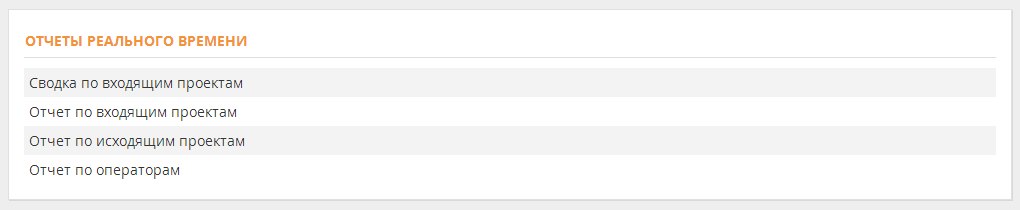
\includegraphics[width=0.85\textwidth]{inc/img/realtime_reports}
    \caption{Отчеты реального времени}
    \label{pic:realtimereports}
\end{figure}

\subsection{Сводки по входящим проектам}

Отчет <<Сводки по входящим проектам>> содержит сводную информацию по выбранным проектам.

\subsection{Отчет по входящим проектам}

\subsection{Отчет по исходящим проектам}

\subsection{Отчет по операторам}

\subsection{График изменения ключевых показателей}

\section{Средства управления}

Управление NCC осуществляется через пользовательский веб-интерфейс, предоставляемый PMS\@.

\section{Сообщения и реакция пользователя} %todo rename

\section{Регламентные работы}

С каждым клиентом отдельно может заключаться договор о технической поддержки, оказываемой со сторны Naumen.

Раз в пол года сотрудниками компании Naumen или ее партнерами проводится проактивное администрирование~\cite{naumen:support}.
В рамках проактивного администрирования осуществляется:
\begin{itemize}
    \item постоянный мониторинг состояния системы и ее компонентов для предотвращения возможных
    инцидентов и проблем;
    \item устранение выявленных при контроле состояния системы потенциальных неисправностей;
    \item предоставление выделенного инженера, владеющего полной информацией о системе, включая
    выполненные доработки, интеграции, примененное сопутствующее ПО и оборудование;
    \item хранение и актуализацию информации о конфигурации информационной системы клиента.
\end{itemize}

По запросу клиента может проводиться удаленное администрирование, либо с вызовом специалиста на место.